\documentclass[ucs]{beamer}
\usepackage{polski}
\usepackage[utf8]{inputenc}
\usepackage{pgfplots}
\usepackage{tikz}
\usetikzlibrary{automata,positioning,shapes,shadows,arrows,backgrounds,trees,fit,calc,decorations.pathreplacing,decorations.markings}

\usetheme{Ilmenau}
%\usetheme{Marburg}

\title{Gas Analyzer \newline aplikacja do analizatorów wykorzystująca protokół ELAN}
\subtitle[Współpraca międzywydziałowa]{Projekt zrealizowany w ramach współpracy między \newline Wydziałem Automatyki, Elektroniki i Informatyki, a \newline Wydziałem Inżynierii Środowiska i Energetyki}

\author[Karbowiak, Powała]{mgr inż. Damian Karbowiak  \and mgr inż. Grzegorz Powała}
\institute[Politechnika Śląska]{
\includegraphics[height=0.2\textheight]{images/PolslLogo} }
\date{\today}
       
\setbeamertemplate{footline}[frame number]
\useoutertheme{infolines}
 
\begin{document}

\begin{frame}
  \titlepage
\end{frame}


\section{Wstęp}
\begin{frame}
\frametitle{Historia}
\begin{itemize}
\setlength{\itemsep}{5pt}
\setlength{\parskip}{5pt}
\setlength{\parsep}{5pt}
\item 22 luty 2013 \\
Kontakt mailowy ze strony mgr inż. Tomasz Kress
\item 28 luty 2013 \\
Pierwsze spotkanie w celu omówienia problemu i zadania
\item 21 marzec 2013 \\
Wypożyczenie Ultramatu 23 i rozpoczęcie współpracy oraz realizacji projektu
\item kwiecień -- czerwiec 2013 \\
Realizacja projektu
\item wrzesień 2013 \\
Finalizacja pierwszej części i podstawowej wersji projektu
\end{itemize}
\end{frame}

\begin{frame}
\frametitle{Współpraca}
\begin{center}
\begin{tabular}{cccccc}

\includegraphics[width=0.1\textwidth]{images/AEiILogo} &

\includegraphics[width=0.1\textwidth]{images/IILogo} &

\includegraphics[width=0.25\textwidth]{images/SKNIndustrumLogo} &

\includegraphics[width=0.1\textwidth]{images/WISiELogo} &

\includegraphics[width=0.1\textwidth]{images/IMIUELogo} &

\includegraphics[width=0.1\textwidth]{images/ZKiWPLogo} \\ 
\end{tabular} 
\end{center}

\begin{enumerate}
\setlength{\itemsep}{3pt}
\setlength{\parskip}{3pt}
\setlength{\parsep}{3pt}
\item Wydział Automatyki, Elektroniki i Informatyki
\begin{itemize}
\setlength{\itemsep}{3pt}
\setlength{\parskip}{3pt}
\setlength{\parsep}{3pt}
\item Instytut Informatyki
\begin{itemize}
\setlength{\itemsep}{3pt}
\setlength{\parskip}{3pt}
\setlength{\parsep}{3pt}
\item Koło Naukowe Przemysłowych Zastosowań Informatyki ,,Industrum''
\\ mgr inż. Damian Karbowiak
\\ mgr inż. Grzegorz Powała
\end{itemize}
\end{itemize}
\item  Wydział Inżynierii Środowiska i Energetyki
\begin{itemize}
\setlength{\itemsep}{3pt}
\setlength{\parskip}{3pt}
\setlength{\parsep}{3pt}
\item Instytut Maszyn i Urządzeń Energetycznych
\begin{itemize}
\setlength{\itemsep}{3pt}
\setlength{\parskip}{3pt}
\setlength{\parsep}{3pt}
\item Zakład Kotłów i Wytwornic Pary
\\ mgr inż. Tomasz Kress
\end{itemize}
\end{itemize}
\end{enumerate}
\end{frame}


\section{Współpraca}
\begin{frame}
\frametitle{Możliwości}
\begin{enumerate}
\setlength{\itemsep}{3pt}
\setlength{\parskip}{3pt}
\setlength{\parsep}{3pt}
\item Instytut Informatyki
\begin{itemize}
\setlength{\itemsep}{2pt}
\setlength{\parskip}{2pt}
\setlength{\parsep}{2pt}
\item Wiedza informatyczna
\item Specjalizacja związana ze stosowaniem informatyki w przemyśle
\item Koło naukowe o tematyce przemysłowej
\item Projekty zaliczeniowe semestralne oraz prace inżynierskie i magisterskie
\item Studenci chętni do realizacji projektów praktycznych z wykorzystaniem istniejącego sprzętu i stanowisk laboratoryjnych
\end{itemize} 
\item Instytut Maszyn i Urządzeń Energetycznych
\begin{itemize}
\setlength{\itemsep}{2pt}
\setlength{\parskip}{2pt}
\setlength{\parsep}{2pt}
\item Potrzeba informatyzacji
\item Ciekawe problemy informatyczne
\item Spora ilość sprzętu i stanowisk
\item Ciekawe pomysły i potrzeby na oprogramowanie/sprzęt
\end{itemize}
\end{enumerate}
\end{frame}

\begin{frame}
\frametitle{Gas Analyzer - geneza}
\begin{enumerate}
\setlength{\itemsep}{5pt}
\setlength{\parskip}{5pt}
\setlength{\parsep}{5pt}
\item Realizacja pomiarów przemysłowych
\item Wykorzystywanie kilku analizatorów firmy SIEMENS
\item Zapisywanie pomiarów w tabelce na kartce
\item Ograniczona częstotliwość pomiarów
\end{enumerate}
\end{frame}

\begin{frame}
\frametitle{Przykładowy wynik pomiarów}
\begin{center}
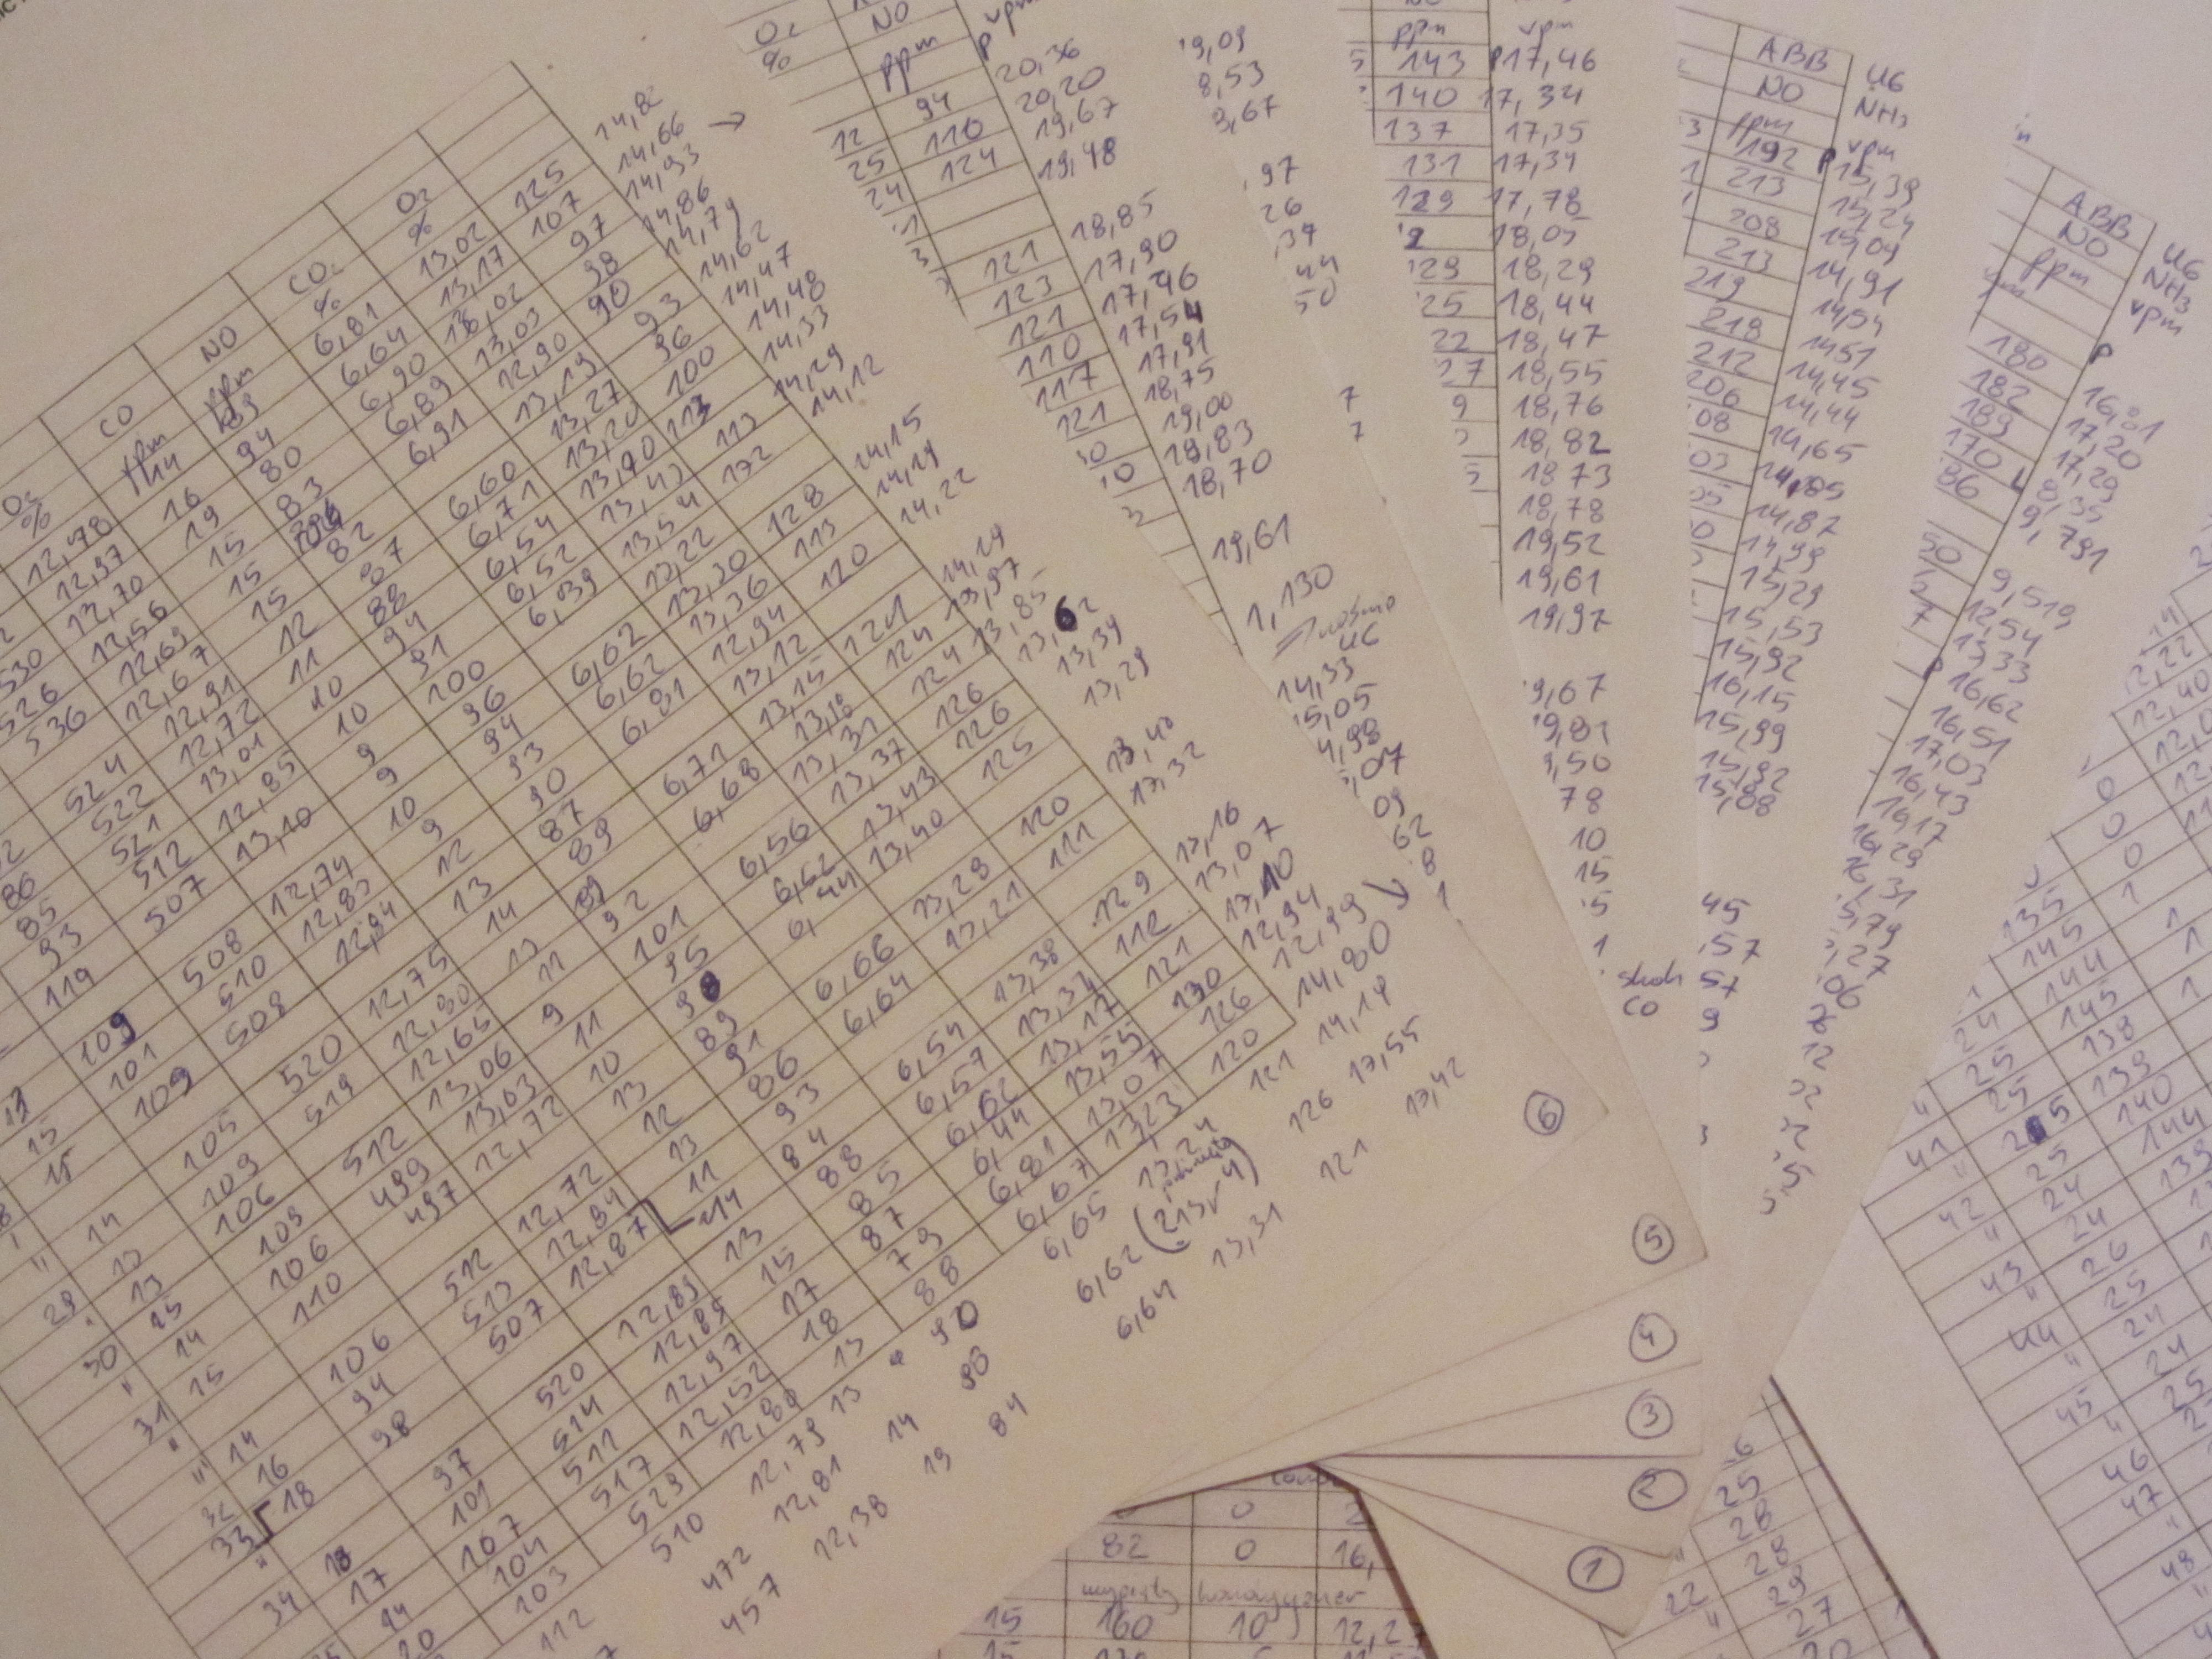
\includegraphics[width=0.99\textheight]{images/IMG_4559}
\end{center}
\end{frame}

\begin{frame}
\frametitle{Przykładowa kartka z pomiarem}
\begin{center}
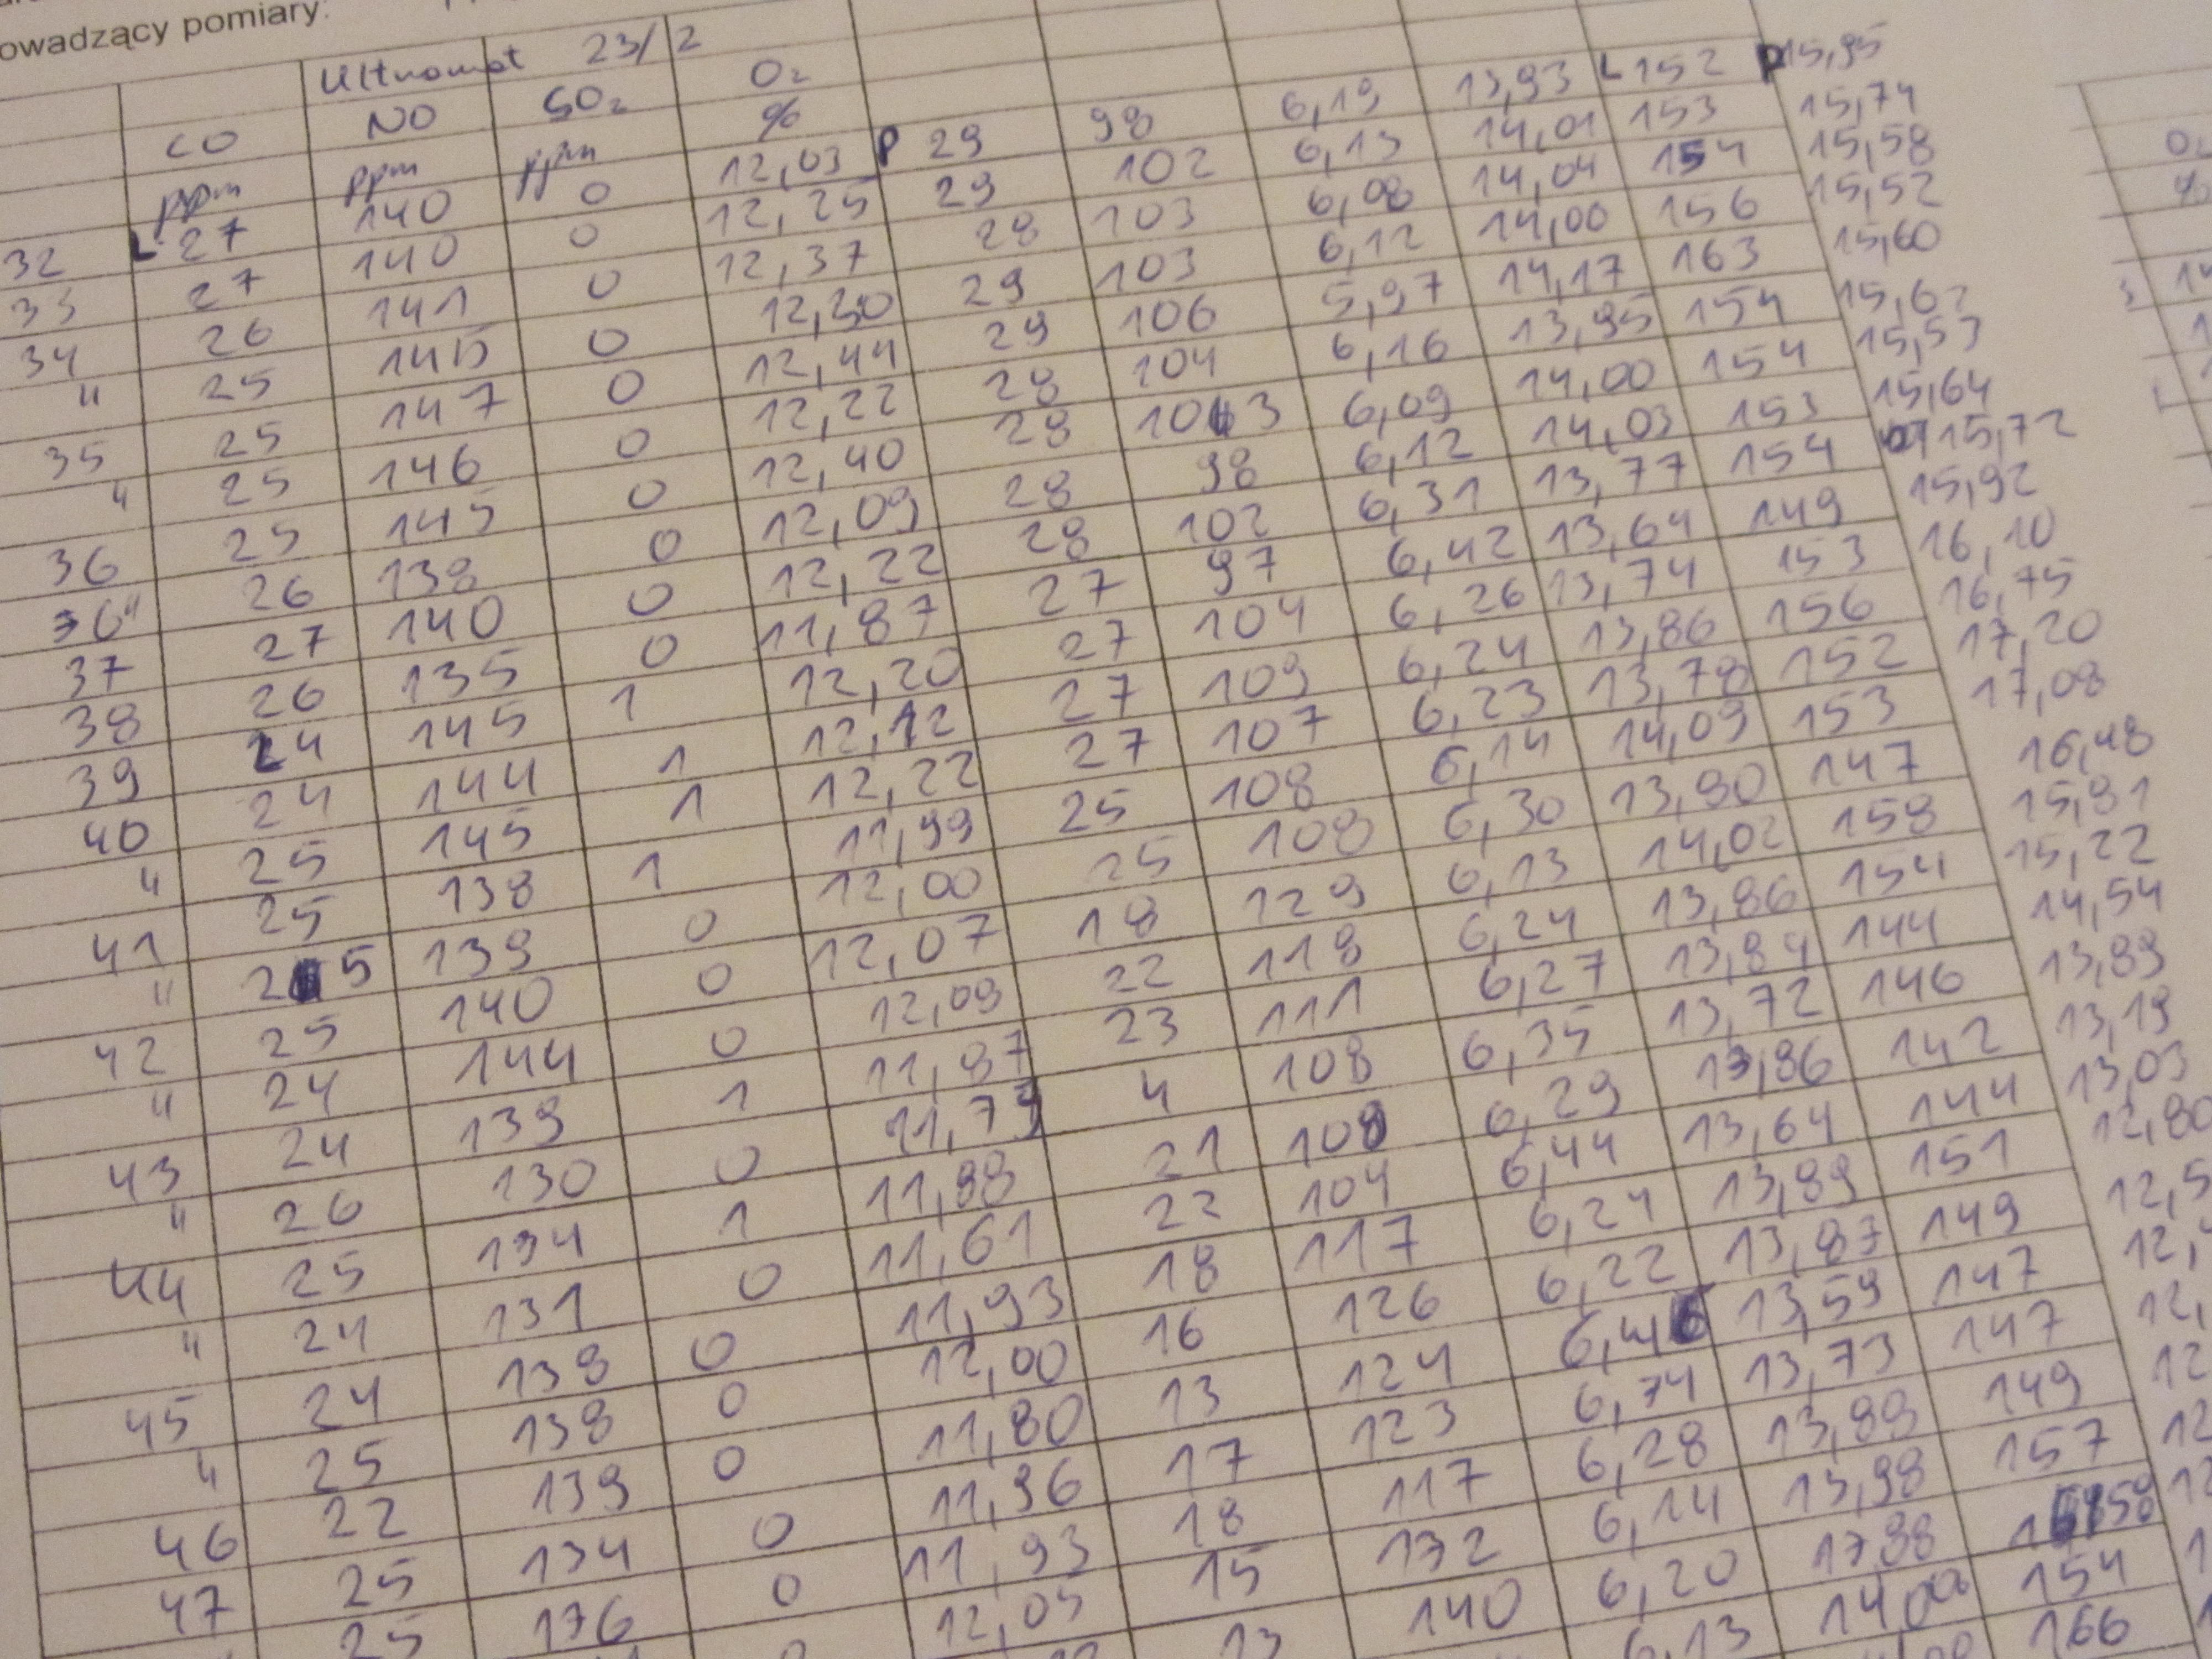
\includegraphics[width=0.99\textheight]{images/IMG_4562}
\end{center}
\end{frame}

\begin{frame}
\frametitle{Gas Analyzer - realizacja}
\begin{enumerate}
\item Wykorzystanie protokołu komunikacyjnego ELAN
\item Możliwość podłączenia do 12 analizatorów firmy SIEMENS:
\begin{itemize}
\item ULTRAMAT 6
\item OXYMAT 6 / OXYMAT 61
\item CALOMAT 6
\item ULTRAMAT 23
\end{itemize}
\item Automatyczny odczyt stanu urządzeń
\item Możliwość archiwizacji pomiarów z dowolnym interwałem czasowym, z~rozdzielczością co sekundę
\item Automatyczne wykrywanie urządzeń i wielkości mierzonych
\item Konfigurowalna precyzja pomiarów (wyświetlanie i raporty)
\item Generowanie raportów do PDF oraz XLS
\item Niskie koszty uruchomienia
\end{enumerate}
\end{frame}

\begin{frame}
\frametitle{ELAN -- Podłączenie}
\tikzstyle{background grid}=[draw, black!50,step=.25cm]
	\begin{tikzpicture}[scale=1]%, show background grid]
	\tikzset{
    	mynode/.style={rectangle,rounded corners,draw=black, top color=white, bottom color=yellow!50,very thick, inner sep=0.5em, minimum size=2em, 		text centered, text width=2.8cm},
	    myarrow/.style={->, >=latex', shorten >=1pt, thick},
	    myline/.style={-, =latex', shorten >=1pt, rounded corners, ultra thick},
	    mylabel/.style={text width=7em, text centered} 
	} 
	\node[mynode] (atc) {Konwerter ATC-850};  
	\node [left=of atc] (laptop) {
\includegraphics[width=3cm]{images/laptop}};

	\node[mynode, below=2cm of atc] (device2) {Urządzenie 2};
	\node[mynode, left=of device2] (device1) {Urządzenie 1};  	 	 	
	\node[mynode, right=of device2] (device12) {Urządzenie 12};	

	\draw[myline,blue] (laptop.east) -- ++(-1, 0) -- (atc.west);

	\draw[myline] (atc.south) -- (device1.north); 
	\draw[myline] (atc.south) -- (device2.north); 
	\draw[myline] (atc.south) -- (device12.north); 		
	\draw[myline, dotted] (device2.east) -- (device12.west); 	
    
	\draw [fill=blue!5, thick] (-5, -5) rectangle (1, -4);

    \draw [blue, line width=6] (-4.5,-4.5) -- (-4,-4.5); \node at (-3.5,-4.5) {USB};
    \draw [black, line width=6] (-2,-4.5) -- (-1.5,-4.5); \node at (-0.8,-4.5) {RS-485};
\end{tikzpicture} 
\end{frame}

\begin{frame}
\frametitle{Podgląd sieci}
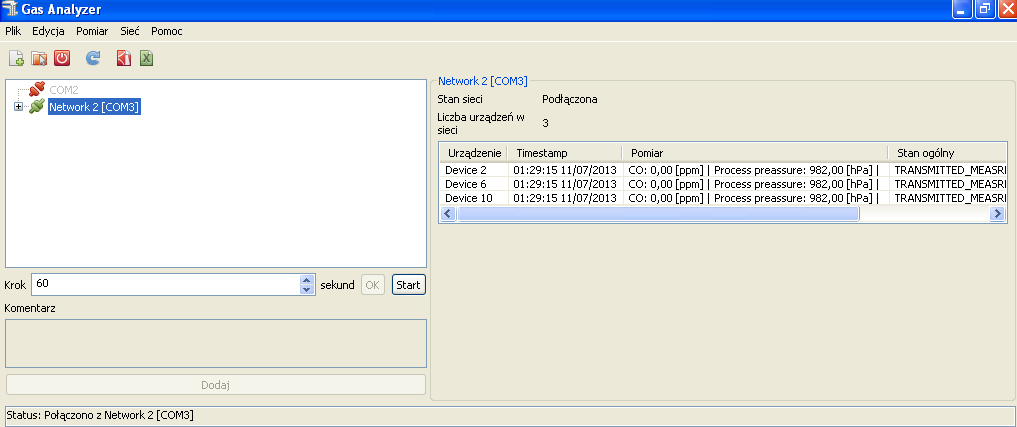
\includegraphics[width=0.99\textwidth]{images/detailNetworkW}
\end{frame}

\begin{frame}
\frametitle{Podgląd urządzenia}
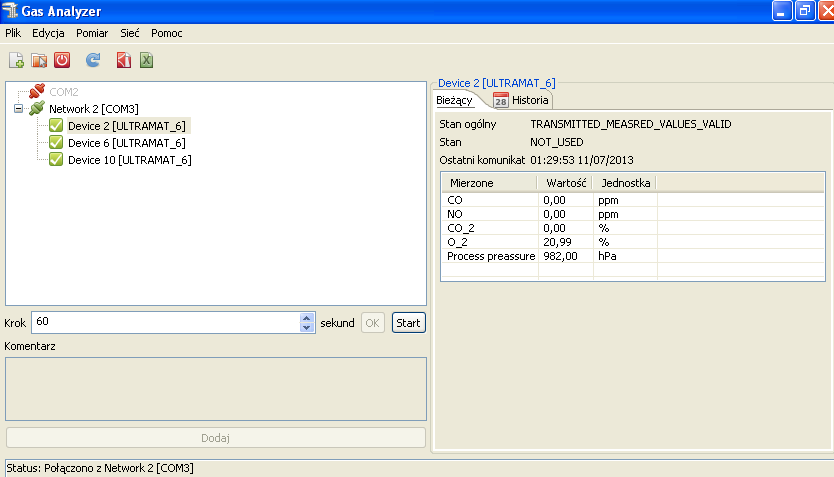
\includegraphics[width=0.99\textwidth]{images/detailDeviceW}
\end{frame}

\begin{frame}
\frametitle{Przykładowy raport PDF}

\includegraphics[width=0.9\textwidth]{images/pdf}
\end{frame}

\begin{frame}
\frametitle{Przykładowy raport XLS}
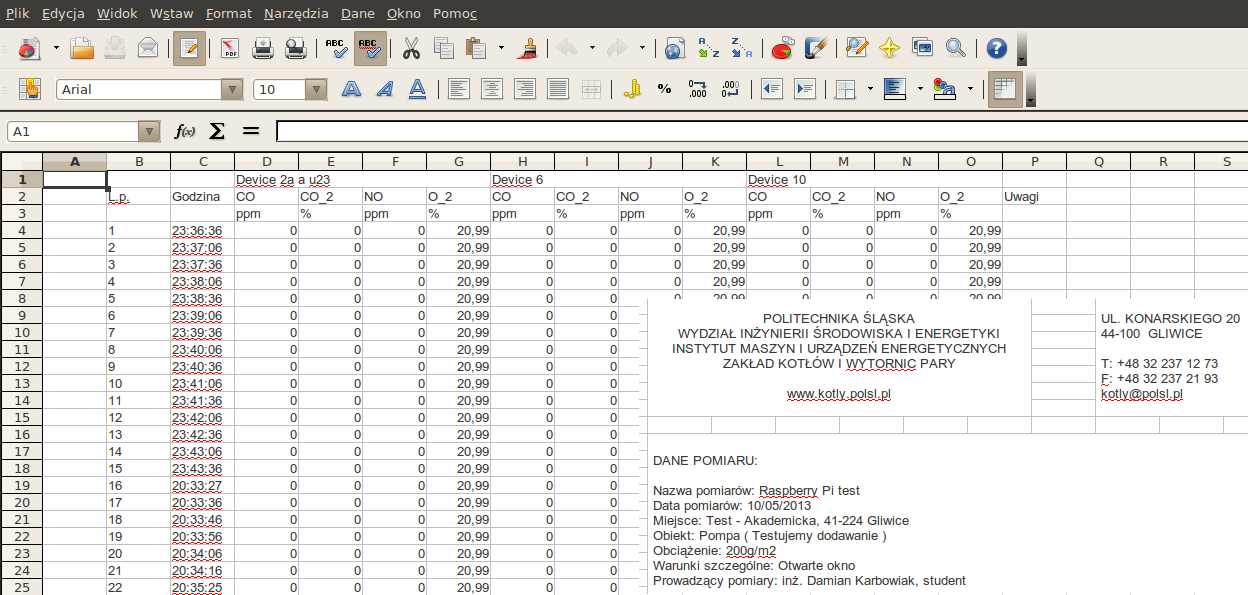
\includegraphics[width=0.99\textwidth]{images/xls}
\end{frame}

\section{Podsumowanie}
\begin{frame}
\frametitle{Wnioski}
\begin{itemize}
\setlength{\itemsep}{5pt}
\setlength{\parskip}{5pt}
\setlength{\parsep}{5pt}
\item Liczne perspektywy współpracy
\item Aktywizacja studentów
\item Rozwiązywanie praktycznych problemów i zadań
\item Utworzenie stałego kanału współpracy 
\item Pozytywne postrzeganie dążenia do współpracy i wymiany doświadczeń
\end{itemize}
\end{frame}

\begin{frame}
\frametitle{Podsumowanie oraz pytania}
Dziękujemy za uwagę.
\\\vspace{2cm}
Czas na pytania.
\\\vspace{2cm}
mgr inż. Damian Karbowiak -- Damian.Karbowiak@polsl.pl\\
mgr inż. Grzegorz Powała -- Grzegorz.Powala@polsl.pl
\end{frame}

\end{document}